%%
%% This is file `sample-sigconf.tex',
%% generated with the docstrip utility.
%%
%% The original source files were:
%%
%% samples.dtx  (with options: `all,proceedings,bibtex,sigconf')
%% 
%% IMPORTANT NOTICE:
%% 
%% For the copyright see the source file.
%% 
%% Any modified versions of this file must be renamed
%% with new filenames distinct from sample-sigconf.tex.
%% 
%% For distribution of the original source see the terms
%% for copying and modification in the file samples.dtx.
%% 
%% This generated file may be distributed as long as the
%% original source files, as listed above, are part of the
%% same distribution. (The sources need not necessarily be
%% in the same archive or directory.)
%%
%%
%% Commands for TeXCount
%TC:macro \cite [option:text,text]
%TC:macro \citep [option:text,text]
%TC:macro \citet [option:text,text]
%TC:envir table 0 1
%TC:envir table* 0 1
%TC:envir tabular [ignore] word
%TC:envir displaymath 0 word
%TC:envir math 0 word
%TC:envir comment 0 0
%%
%%
%% The first command in your LaTeX source must be the \documentclass
%% command.
%%
%% For submission and review of your manuscript please change the
%% command to \documentclass[manuscript, screen, review]{acmart}.
%%
%% When submitting camera ready or to TAPS, please change the command
%% to \documentclass[sigconf]{acmart} or whichever template is required
%% for your publication.
%%
%%
\documentclass[sigconf]{acmart}

%%
%% \BibTeX command to typeset BibTeX logo in the docs
\AtBeginDocument{%
  \providecommand\BibTeX{{%
    Bib\TeX}}}

%% Rights management information.  This information is sent to you
%% when you complete the rights form.  These commands have SAMPLE
%% values in them; it is your responsibility as an author to replace
%% the commands and values with those provided to you when you
%% complete the rights form.
\setcopyright{acmlicensed}
\copyrightyear{2018}
\acmYear{2018}
\acmDOI{XXXXXXX.XXXXXXX}

%% These commands are for a PROCEEDINGS abstract or paper.
\acmConference[Conference acronym 'XX]{Make sure to enter the correct
  conference title from your rights confirmation emai}{June 03--05,
  2018}{Woodstock, NY}
%%
%%  Uncomment \acmBooktitle if the title of the proceedings is different
%%  from ``Proceedings of ...''!
%%
%%\acmBooktitle{Woodstock '18: ACM Symposium on Neural Gaze Detection,
%%  June 03--05, 2018, Woodstock, NY}
\acmISBN{978-1-4503-XXXX-X/18/06}


%%
%% Submission ID.
%% Use this when submitting an article to a sponsored event. You'll
%% receive a unique submission ID from the organizers
%% of the event, and this ID should be used as the parameter to this command.
%%\acmSubmissionID{123-A56-BU3}

%%
%% For managing citations, it is recommended to use bibliography
%% files in BibTeX format.
%%
%% You can then either use BibTeX with the ACM-Reference-Format style,
%% or BibLaTeX with the acmnumeric or acmauthoryear sytles, that include
%% support for advanced citation of software artefact from the
%% biblatex-software package, also separately available on CTAN.
%%
%% Look at the sample-*-biblatex.tex files for templates showcasing
%% the biblatex styles.
%%

%%
%% The majority of ACM publications use numbered citations and
%% references.  The command \citestyle{authoryear} switches to the
%% "author year" style.
%%
%% If you are preparing content for an event
%% sponsored by ACM SIGGRAPH, you must use the "author year" style of
%% citations and references.
%% Uncommenting
%% the next command will enable that style.
%%\citestyle{acmauthoryear}

% my packages
\usepackage{paralist}


\makeatletter
\newcommand\bigscriptsize{\@setfontsize\bigscriptsize\@viiipt\@ixpt}
\makeatother

\newcommand{\Hquad}{\hspace{0.5em}}
\newcommand{\HHquad}{\hspace{0.25em}}

\DeclareMathOperator{\val}{=}  % for p=v atoms
\DeclareMathOperator{\nval}{{\neq}}  % for p=v atoms

\def\happensAt{\textsf{\bigscriptsize happensAt}}
\def\happens{\textsf{\bigscriptsize happensAt}}
\def\initially{\textsf{\bigscriptsize initially}}
\def\holds{\textsf{\bigscriptsize holds}}
\def\notholds{\textsf{\bigscriptsize notholds}}
\def\holdsAt{\textsf{\bigscriptsize holdsAt}}
\def\holdsAtEC{\textsf{\bigscriptsize holdsAtEC}}
\def\holdsAtCyclic{\textsf{\bigscriptsize holdsAtCyclic}}
\def\holdsAtProcessed{\textsf{\bigscriptsize holdsAtProcessed}}
\def\holdsFor{\textsf{\bigscriptsize holdsFor}}
\def\initiatedAt{\textsf{\bigscriptsize initiatedAt}}
\def\terminatedAt{\textsf{\bigscriptsize terminatedAt}}
\def\broken{\textsf{\bigscriptsize broken}}
\def\brokenAt{\textsf{\bigscriptsize brokenAt}}
\def\brokenBetween{\textsf{\bigscriptsize brokenBetween}}
\def\updateCache{\textsf{\bigscriptsize updateCache}}
\def\startE{\textsf{\bigscriptsize start}}
\def\endE{\textsf{\bigscriptsize end}}
\def\processed{\textsf{\bigscriptsize processed}}
\def\cachedPoints{\textsf{\bigscriptsize cachedLEQ}}
\def\inCachedPoints{\textsf{\bigscriptsize inCachedPoints}}
\def\startedAt{\textsf{\bigscriptsize startedAt}}
\def\endedAt{\textsf{\bigscriptsize endedAt}}
\def\maxDuration{\textsf{\bigscriptsize fi}}
\def\extensible{\textsf{\bigscriptsize p}}
\def\startedBetween{\textsf{\bigscriptsize startedBetween}}
\def\brokenBetween{\textsf{\bigscriptsize brokenBetween}}
\def\cancelled{\textsf{\bigscriptsize cancelled}}
\def\happensStartOrHolds{\textsf{\bigscriptsize happensStartOrHolds}}
\def\happensEndOrNotHolds{\textsf{\bigscriptsize happensEndOrNotHolds}}
\def\positiveOrNegative{\textsf{\bigscriptsize positiveOrNegativeCond}}
\def\notHoldsAndNotStarts{\textsf{\bigscriptsize notHoldsAndNotStarts}}
\def\holdsAndNotEnds{\textsf{\bigscriptsize holdsAndNotEnds}}
\def\algfor{\textsf{\bigscriptsize for}}

\def\allen{\textsf{\bigscriptsize allen}}
\def\before{\textsf{\bigscriptsize before}}
\def\beforeInv{\textsf{\bigscriptsize before\_inverse}}
\def\meets{\textsf{\bigscriptsize meets}}
\def\meetsInv{\textsf{\bigscriptsize meets\_inverse}}
\def\starts{\textsf{\bigscriptsize starts}}
\def\startsInv{\textsf{\bigscriptsize starts\_inverse}}
\def\finishes{\textsf{\bigscriptsize finishes}}
\def\finishesInv{\textsf{\bigscriptsize finishes\_inverse}}
\def\during{\textsf{\bigscriptsize during}}
\def\duringInv{\textsf{\bigscriptsize during\_inverse}}
\def\overlaps{\textsf{\bigscriptsize overlaps}}
\def\overlapsInv{\textsf{\bigscriptsize overlaps\_inverse}}
\def\equal{\textsf{\bigscriptsize equal}}
\def\lhs{\textsf{\bigscriptsize source}}
\def\rhs{\textsf{\bigscriptsize target}}
\def\union{\textsf{\bigscriptsize union}}
\def\intersect{\textsf{\bigscriptsize intersect}}
\def\complement{\textsf{\bigscriptsize complement\_all}}
\def\complementInv{\textsf{\bigscriptsize complement\_inv}}

\def\holdsshort{\textsf{\bigscriptsize h}}
\def\initshort{\textsf{\bigscriptsize init}}
\def\termshort{\textsf{\bigscriptsize term}}

\def\nbf{\textsf{\bigscriptsize not}}
\def\true{\textsf{\bigscriptsize true}}
\def\false{\textsf{\bigscriptsize false}}
\def\tval{\textsf{\bigscriptsize tval}}
\def\fval{\textsf{\bigscriptsize fval}}

\def\fv{$\mathit{F{=}V}$}
\def\fvprime{$\mathit{F'\val V'}$}
\def\fvprimediff{$\mathit{F'\val V''}$}
\def\nequiv{\not\equiv}
\def\dlt{$\mathit{T{+}R}$}
\def\fvdiff{$\mathit{F\val V'}$}

%\def\sfluent{F^{sf}}
\def\sfluent{F}
\def\sfv{\sfluent\val V}
%\def\sdfluent{F^{sdf}}
\def\sdfluent{F}
\def\sdfv{\sdfluent\val V}
\def\intervalsymb{J}

\newcommand{\sfvno}[1]{\sfluent_{#1}\val V_{#1}}
\newcommand{\sdfvno}[1]{\sdfluent_{#1}\val V_{#1}}

\def\prevtp{prev}
\def\nexttp{next}
\def\isstartingpoint{isStartingPoint}
\def\isendingpoint{isEndingPoint}

\def\unionall{\textsf{\bigscriptsize union\_all}}
\def\intersectall{\textsf{\bigscriptsize intersect\_all}}
\def\complementall{\textsf{\bigscriptsize relative\_complement\_all}}
\def\atemporalconstraints{\textit{atemporal\_constraints}}
\def\intervalManipulation{\textsf{\bigscriptsize intervalConstruct}}
\def\durationGreater{\textsf{\bigscriptsize duration\_greater}}
\def\durationLess{\textsf{\bigscriptsize duration\_less}}

\def\RTEC{$\mathit{RTEC}$}
\def\RTECcyc{RTEC$_{\circ}$}
\def\RTECcycnaive{RTEC$_{\circ}$-naive}
\def\rd{RTEC$^{\rightarrow}$}
\def\rtec{RTEC}
\def\RTECWM{$\mathit{RTEC_{\omega}}$}
\def\ed{R^{\text{\rd}}}
\def\partord{{\prec}}
\def\npartord{{\nprec}}
\def\procord{{\partord^*}}
\def\nprocord{{\npartord^*}}
\def\vertices{\mathcal{V}}
\def\edges{\mathcal{E}}
\def\minus{{-}}
\def\plus{{+}}
\def\iff{\leftrightarrow}

\def\qeddef{\hfill $\blacksquare$}
\def\qedex{\hfill $\lozenge$}
\def\qedprop{\hfill $\blacklozenge$}
\def\qedlem{\hfill $\blacktriangle$}
\def\qedcor{\hfill $\triangle$}
\def\qedproof{\hfill $\square$}

\def\iedge{i-edge}
\def\fedge{f-edge}
\def\iedges{\edges_{i}}
\def\futedges{\edges_{f}}

\def\levelstruct{FVPs\_per\_level\_map}
\def\cyclestruct{maximal\_cycles}

\newcommand{\fluentgraph}[1]{G^{#1}}
\newcommand{\fluentvertices}[1]{\vertices^{#1}}
\newcommand{\fluentiedges}[1]{\iedges^{#1}}
\newcommand{\fluentfedges}[1]{\futedges^{#1}}

\def\preord{\prec}
\def\npreord{\nprec}
\def\procord{\preord^*}
\def\nprocord{\npreord^*}

\newcommand{\preordarg}[1]{\prec_{#1}}
\newcommand{\npreordarg}[1]{\nprec_{#1}}
\newcommand{\procordarg}[1]{\preord^*_{#1}}
\newcommand{\nprocordarg}[1]{\npreord^*_{#1}}

\def\rtecallen{\texorpdfstring{RTEC\textsubscript{A}}{RTECa}}
\def\rel{\textsf{\bigscriptsize rel}}
\def\intList{I}
\def\intOp{\textsf{\bigscriptsize outMode}}
\newcommand{\intListi}[1]{i_{#1}}
\def\slist{\mathcal{S}}
\def\tlist{\mathcal{T}}
\def\sint{i^s}
\def\tint{i^t}

\newcommand{\beforeRel}[2]{\mathit{\before(#1,#2)}}
\newcommand{\beforeInvRel}[2]{\mathit{\beforeInv(#1,#2)}}
\newcommand{\meetsRel}[2]{\mathit{\meets(#1,#2)}}
\newcommand{\meetsInvRel}[2]{\mathit{\meetsInv(#1,#2)}}

\newcommand{\startsRel}[2]{\mathit{\starts(#1,#2)}}
\newcommand{\startsInvRel}[2]{\mathit{\startsInv(#1,#2)}}
\newcommand{\finishesRel}[2]{\mathit{\finishes(#1,#2)}}
\newcommand{\finishesInvRel}[2]{\mathit{\finishesInv(#1,#2)}}

\newcommand{\duringRel}[2]{\mathit{\during(#1,#2)}}
\newcommand{\duringInvRel}[2]{\mathit{\duringInv(#1,#2)}}
\newcommand{\overlapsRel}[2]{\mathit{\overlaps(#1,#2)}}
\newcommand{\overlapsInvRel}[2]{\mathit{\overlapsInv(#1,#2)}}

\newcommand{\equalRel}[2]{\mathit{\equal(#1,#2)}}

\newcommand{\relRel}[2]{\mathit{\rel(#1,#2)}}
\newcommand{\relInvRel}[2]{\mathit{\relInv(#1,#2)}}
\newcommand{\satrelRel}[2]{\mathit{\satrel(#1,#2)}}

\newcommand{\allenPred}[5]{\mathit{\allen(#1,#2,#3,#4,#5)}}

\newcommand{\beforePred}[4]{\mathit{\before(#1,#2,#3,#4)}}
\newcommand{\beforeInvPred}[4]{\mathit{\beforeInv(#1,#2,#3,#4)}}
\newcommand{\meetsPred}[4]{\mathit{\meets(#1,#2,#3,#4)}}
\newcommand{\meetsInvPred}[4]{\mathit{\meetsInv(#1,#2,#3,#4)}}

\newcommand{\startsPred}[4]{\mathit{\starts(#1,#2,#3,#4)}}
\newcommand{\startsInvPred}[4]{\mathit{\startsInv(#1,#2,#3,#4)}}
\newcommand{\finishesPred}[4]{\mathit{\finishes(#1,#2,#3,#4)}}
\newcommand{\finishesInvPred}[4]{\mathit{\finishesInv(#1,#2,#3,#4)}}

\newcommand{\duringPred}[4]{\mathit{\during(#1,#2,#3,#4)}}
\newcommand{\duringInvPred}[4]{\mathit{\duringInv(#1,#2,#3,#4)}}
\newcommand{\overlapsPred}[4]{\mathit{\overlaps(#1,#2,#3,#4)}}
\newcommand{\overlapsInvPred}[4]{\mathit{\overlapsInv(#1,#2,#3,#4)}}

\newcommand{\equalPred}[4]{\mathit{\equal(#1,#2,#3,#4)}}

\newcommand{\relPred}[4]{\mathit{\rel(#1,#2,#3,#4)}}
\newcommand{\relInvPred}[4]{\mathit{\relInv(#1,#2,#3,#4)}}

\newcommand{\eventsdf}[1]{#1^{sdf}}
\def\timepoints{\mathbb{T}}

\newcommand{\compl}[1]{\overline{#1}}
\newcommand{\symm}[1]{\overline{#1}}
\def\subst{\triangleleft}
\def\append{\textsf{\bigscriptsize add}}

\def\edgespast{\edges^{past}}
\def\edgesconc{\edges^{conc}}

\def\fvpsubst{\sigma}
\def\fvpset{\mathcal{F}}
\def\ordersymm{\mathbb{O}}
\newcommand{\ordersymmetric}[1]{\ordersymm_{#1}}
\def\orderflip{fl}
\def\fvps{fvps}
\def\intervalprops{v}

\def\fgraph{G^{fl}}
\def\fvertices{\vertices^{fl}}
\def\fedges{\edges^{fl}}

\def\cdfdg{G^{cdfl}}
\def\contractedfdg{\cdfdg}
\def\cdfvertices{\vertices^{cdfl}}
\def\verticescontracted{\cdfvertices}
\def\cdfedges{\edges^{cdfl}}
\def\edgescontracted{\cdfedges}
\def\hvals{hvals}

\def\cdg{G^c}
\def\cvertices{\vertices^c}
\def\cedges{\edges^c}

\newcommand{\initvertex}[1]{v^{init}_{#1}}
\newcommand{\termvertex}[1]{v^{term}_{#1}}
\def\nextI{next}

\def\fvpordered{FVP-ordered}

\def\condset{IC}
\def\guardset{G}
\newcommand{\guardseti}[1]{\guardset^{#1}}
\newcommand{\guardsetemi}[1]{\guardset^{e#1}_m}
\newcommand{\guardsetemgi}[1]{\guardset'^{e#1}_m}

\def\guardfuncs{g}
\def\guardfunce{ge}
\def\tupletointname{\pi}
\newcommand{\tupletoint}[1]{\tupletointname^{(#1)}}

\def\funcset{\mathcal{F}}

\def\initset{R^s}
\def\termset{R^e}
\newcommand{\initseti}[1]{R^{s#1}}
\newcommand{\termseti}[1]{R^{e#1}}
\def\initsetm{\initset_m}
\newcommand{\initsetmi}[1]{R^{s#1}_m}
\def\termsetm{\termset_m}
\newcommand{\termsetmi}[1]{R^{e#1}_m}
\def\termsetmg{R'^e_m}
\newcommand{\termsetmgi}[1]{R'^{e#1}_m}
\def\boolm{p_m}
\def\statm{r_m}

\def\compilerarrow{\rightsquigarrow}

\makeatletter
\newcommand*{\bdiv}{%
  \nonscript\mskip-\medmuskip\mkern5mu%
  \mathbin{\operator@font div}\penalty900\mkern5mu%
  \nonscript\mskip-\medmuskip
}
\makeatother

\def\eventdesc{\mathcal{E}}
\newcommand{\edarg}[1]{\eventdesc_{#1}}
\def\edsf{\eventdesc^{i}}
\newcommand{\edsfarg}[1]{\edsf_{#1}}
\def\edsdf{\eventdesc^{o}}
\newcommand{\edsdfarg}[1]{\edsdf_{#1}}
\newcommand{\edsfg}[1]{\eventdesc^{sf.{#1}}}
\newcommand{\edsfgarg}[2]{\edsfg{#1}_{#2}}

% mathit everywhere
\everymath{\it}\everydisplay{\it}

% set emergencystretch to avoid margin overflows for inline math.
%\setlength\emergencystretch{\hsize}

%\newtheoremstyle{theoremdd}% name of the style to be used
%  {\topsep}% measure of space to leave above the theorem. E.g.: 3pt
%  {\topsep}% measure of space to leave below the theorem. E.g.: 3pt
%  {\normalfont}%{\itshape}% name of font to use in the body of the theorem
%  {0pt}% measure of space to indent
%  {\bfseries}% name of head font
%  {:}% punctuation between head and body
%  { }% space after theorem head; " " = normal interword space
%  {\thmname{#1}\thmnumber{ #2}\thmnote{ (#3)}}

%\theoremstyle{theoremdd}

\newtheoremstyle{mytheoremkr}% name of the style to be used
  {3pt}% measure of space to leave above the theorem. E.g.: 3pt
  {3pt}% measure of space to leave below the theorem. E.g.: 3pt
  {\normalfont}%{\itshape}% name of font to use in the body of the theorem
  {0pt}% measure of space to indent
  {\bfseries}% name of head font
  {.}% punctuation between head and body
  { }% space after theorem head; " " = normal interword space
  {}

\theoremstyle{mytheoremkr}

% See https://www.overleaf.com/learn/latex/theorems_and_proofs
% for a nice explanation of how to define new theorems, but keep
% in mind that the amsthm package is already included in this
% template and that you must *not* alter the styling.
\newtheorem{example}{Example}
\newtheorem{theorem}{Theorem}
\newtheorem{definition}{Definition}
\newtheorem{proposition}{Proposition}
\newtheorem{lemma}{Lemma}
\newtheorem{corollary}{Corollary}

\newtheoremstyle{myproof}% name of the style to be used
  {3pt}% measure of space to leave above the theorem. E.g.: 3pt
  {3pt}% measure of space to leave below the theorem. E.g.: 3pt
  {\normalfont}%{\itshape}% name of font to use in the body of the theorem
  {0pt}% measure of space to indent
  {\bfseries}% name of head font
  {.}% punctuation between head and body
  { }% space after theorem head; " " = normal interword space
  {}

\theoremstyle{myproof}
\newtheorem*{proofsketch}{Proof Sketch}

\newenvironment{mysplit}%
  {\arraycolsep 0pt \begin{array}{l}}%
  {\end{array}}

\newenvironment{logicrule}%
  {\begin{equation}\begin{array}{l}}%
  {\end{array}\end{equation}}

\newenvironment{logicrulenn}%
  {\begin{equation*}\begin{array}{l}}%
  {\end{array}\end{equation*}}

% Algpseudocode command to create sub-algorithms
\newcommand\Algphase[1]{% 
\vspace*{-.5\baselineskip}\Statex\hspace*{\dimexpr-\algorithmicindent-2pt\relax}%\hrule% 
\Statex\hspace*{-\algorithmicindent}#1% 
\vspace*{-.7\baselineskip}\Statex\hspace*{\dimexpr-\algorithmicindent-2pt\relax}%\hrule%
}

% for align to span multiple pages/columns
\allowdisplaybreaks


%%
%% end of the preamble, start of the body of the document source.
\begin{document}

%%
%% The "title" command has an optional parameter,
%% allowing the author to define a "short title" to be used in page headers.
\title{Composite Activity Definition Construction with Large Larnguage Models}
%%
%% The "author" command and its associated commands are used to define
%% the authors and their affiliations.
%% Of note is the shared affiliation of the first two authors, and the
%% "authornote" and "authornotemark" commands
%% used to denote shared contribution to the research.
\author{Andreas Kouvaras}
\email{a.kouvaras@unipi.gr}
\affiliation{%
  \institution{University of Piraeus}
  %\city{Dublin}
  %\state{Ohio}
  \country{Greece}
}

\author{Periklis Mantenoglou}
\email{pmantenoglou@iit.demokritos.gr}
\orcid{0009-0002-3275-1522}
\affiliation{%
  \institution{NCSR ``Demokritos''}
  %\city{Hekla}
  \country{Greece}}

\author{Alexander Artikis}
\email{a.artikis@unipi.gr}
\orcid{0000-0001-6899-4599}
\affiliation{%
  \institution{University of Piraeus \& NCSR ``Demokritos''}
  \country{Greece}
}
%%
%% By default, the full list of authors will be used in the page
%% headers. Often, this list is too long, and will overlap
%% other information printed in the page headers. This command allows
%% the author to define a more concise list
%% of authors' names for this purpose.
\renewcommand{\shortauthors}{Kouvaras et al.}

%%
%% The abstract is a short summary of the work to be presented in the
%% article.
\begin{abstract}
  We use LLMs to construct event descriptions for RTEC.
\end{abstract}

%%
%% The code below is generated by the tool at http://dl.acm.org/ccs.cfm.
%% Please copy and paste the code instead of the example below.
%%
\begin{CCSXML}
<ccs2012>
 <concept>
  <concept_id>00000000.0000000.0000000</concept_id>
  <concept_desc>Do Not Use This Code, Generate the Correct Terms for Your Paper</concept_desc>
  <concept_significance>500</concept_significance>
 </concept>
 <concept>
  <concept_id>00000000.00000000.00000000</concept_id>
  <concept_desc>Do Not Use This Code, Generate the Correct Terms for Your Paper</concept_desc>
  <concept_significance>300</concept_significance>
 </concept>
 <concept>
  <concept_id>00000000.00000000.00000000</concept_id>
  <concept_desc>Do Not Use This Code, Generate the Correct Terms for Your Paper</concept_desc>
  <concept_significance>100</concept_significance>
 </concept>
 <concept>
  <concept_id>00000000.00000000.00000000</concept_id>
  <concept_desc>Do Not Use This Code, Generate the Correct Terms for Your Paper</concept_desc>
  <concept_significance>100</concept_significance>
 </concept>
</ccs2012>
\end{CCSXML}

\ccsdesc[500]{Do Not Use This Code~Generate the Correct Terms for Your Paper}
\ccsdesc[300]{Do Not Use This Code~Generate the Correct Terms for Your Paper}
\ccsdesc{Do Not Use This Code~Generate the Correct Terms for Your Paper}
\ccsdesc[100]{Do Not Use This Code~Generate the Correct Terms for Your Paper}

%%
%% Keywords. The author(s) should pick words that accurately describe
%% the work being presented. Separate the keywords with commas.
\keywords{Do, Not, Us, This, Code, Put, the, Correct, Terms, for,
  Your, Paper}
%% A "teaser" image appears between the author and affiliation
%% information and the body of the document, and typically spans the
%% page.
%\begin{teaserfigure}
  %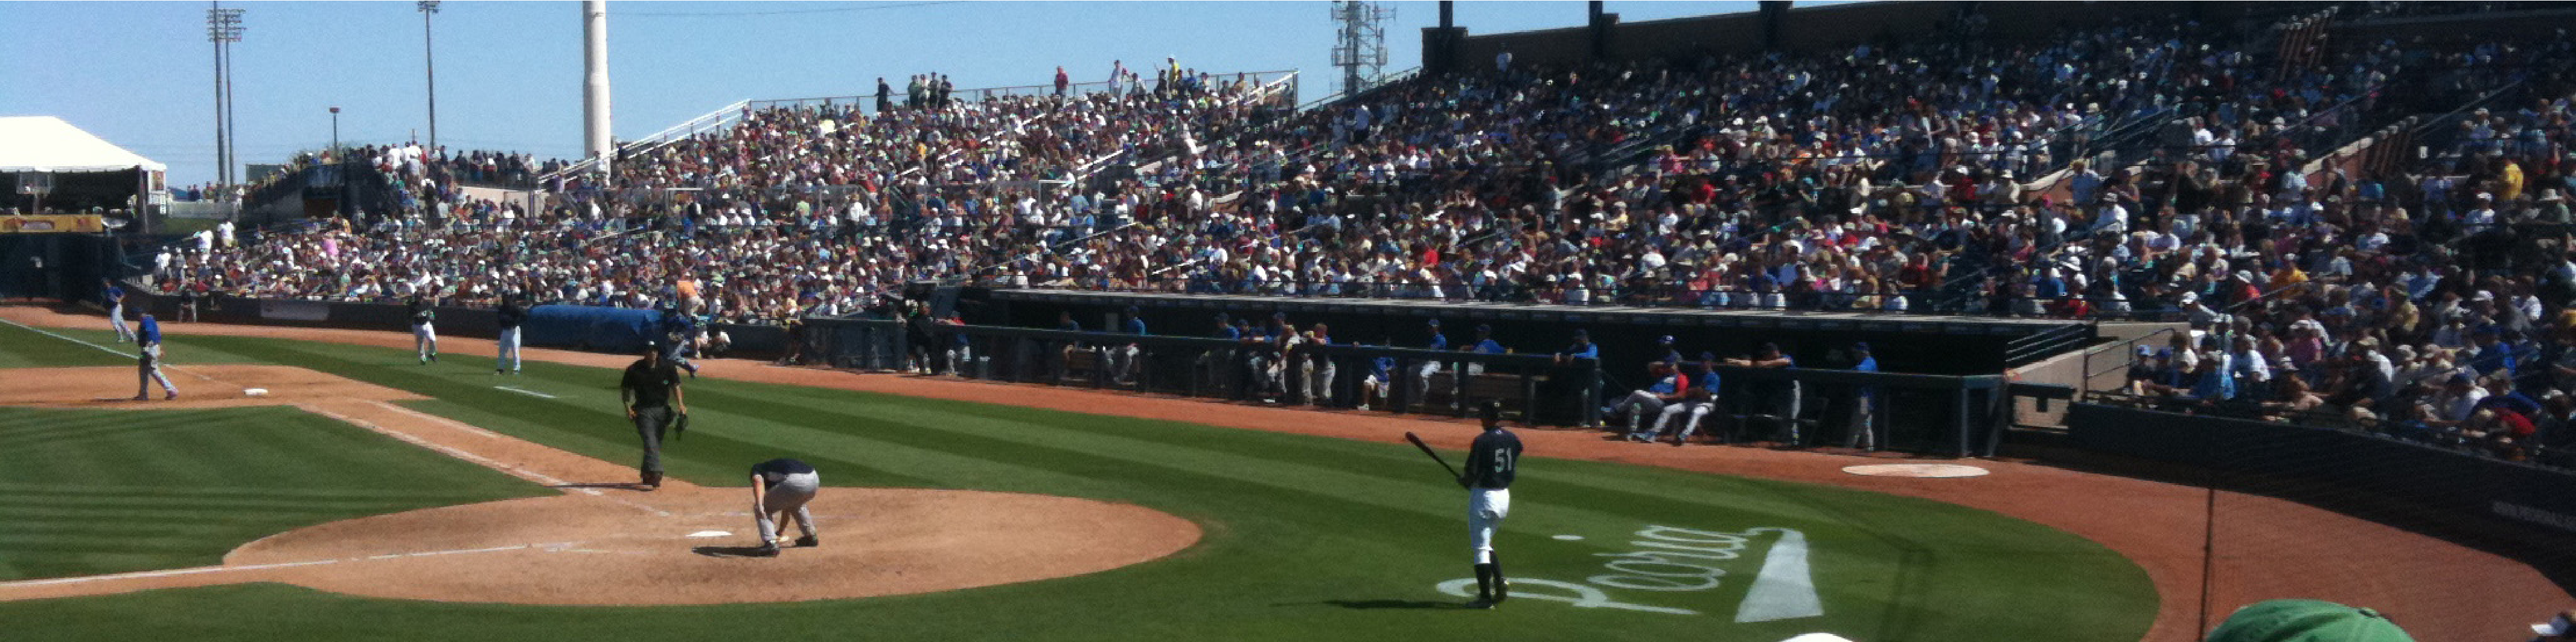
\includegraphics[width=\textwidth]{sampleteaser}
  %\caption{Seattle Mariners at Spring Training, 2010.}
  %\Description{Enjoying the baseball game from the third-base
  %seats. Ichiro Suzuki preparing to bat.}
  %\label{fig:teaser}
%\end{teaserfigure}

\received{20 February 2007}
\received[revised]{12 March 2009}
\received[accepted]{5 June 2009}

%%
%% This command processes the author and affiliation and title
%% information and builds the first part of the formatted document.
\maketitle

\section{Introduction}\label{sec:intro}


\section{Background}\label{sec:background}

\subsection{Run-Time Event Calculus}

The Event Calculus is a logic programming formalisms for representing events and reasoning about their effects over time~\cite{kowalski86}.
%
The Run-Time Event Calculus (\rtec) is an extension of the Event Calculus that is optimised for composite event recognition over large event streams~\cite{DBLP:journals/tkde/ArtikisSP15,DBLP:conf/kr/MantenoglouPA22,DBLP:conf/kr/MantenoglouKA23}.

\textbf{Representation.}~The language of \rtec\ is many-sorted, including sorts for representing time, instantaneous events and fluents. %', i.e., properties whose value may change over time.
%
\rtec\ employs a linear time-line with non-negative integer time-points.
%Event occurrences may change the values of fluents.
%
A `fluent-value pair' (FVP) \fv\ denotes that fluent $F$ has value $V$.
%
%Boolean fluents are a special case where the possible values are $\true$ and $\false$.
%
%We call \fv\ a `fluent-value pair' (FVP).
%
%
%We describe the main predicates of \rtec.
%
$\happensAt(E, T)$ signifies that event $E$ occurs at time-point $T$.
%
$\initiatedAt(F\val V, T)$ (resp.~$\terminatedAt(F\val V, T)$) expresses that a time period during which a fluent $F$ has the value $V$ continuously is initiated (terminated) at $T$.
%
$\holdsAt(F\val V, T)$ states that $F$ has value $V$ at $T$, while $\holdsFor(F\val V, I)$ expresses that \fv\ holds continuously in the intervals included in list $I$.

A formalisation of the temporal specifications of a domain in \rtec\ is called \emph{event description}.
%
\begin{definition}[Event Description]\label{def:event_description}
An event description is a set of:
%
\begin{compactitem}
\item ground $\happensAt(E, T)$ facts, expressing an input stream of event instances, 
\item rules with head $\initiatedAt(F\val V, T)$ or $\terminatedAt(F\val V, T)$, expressing the effects of events on FVP \fv, and
\item rules with head $\holdsFor(F\val V, I)$, defining FVP \fv\ based on other FVPs. \qeddef  % in terms of other FVPs. \qeddef
\end{compactitem}
%
\end{definition}

\rtec\ features two types of FVPs: `simple' and `statically determined'.
%
Simple FVPs are defined using a set of $\initiatedAt$ and $\terminatedAt$ rules, and are subject to the commonsense law of inertia, i.e., a FVP \fv\ holds at a time-point $T$, if \fv\ has been `initiated' by an event at a time-point earlier than $T$, and not `terminated' by another event in the meantime.  

% Maritime Example % 

\begin{example}[Within area]\label{ex:withinarea}
%
In maritime monitoring, various areas, e.g., fisheries restricted areas, disallow certain activities.
%
It is thus useful to compute the intervals during which a vessel is in such an area.
%
See the formalisation below:
%
\begin{align}
& \label{eq:withinArea-init}
\begin{mysplit}
\mathit{\initiatedAt(withinArea(Vl,AreaType)\val\true,T)} \leftarrow \\
	\quad\mathit{\happensAt(entersArea(Vl,AreaID),T),} \\
	\quad\mathit{areaType(AreaID,AreaType).}
\end{mysplit}\\
& \label{eq:withinArea-term}
\begin{mysplit} 
\mathit{\terminatedAt(withinArea(Vl,AreaType)\val\true,T)} \leftarrow \\
	\quad\mathit{\happensAt(leavesArea(Vl,AreaID), T),} \\
	\quad\mathit{areaType(AreaID,AreaType).} 
\end{mysplit}\\
& \label{eq:withinArea-term2}
\begin{mysplit} 
\mathit{\terminatedAt(withinArea(Vl,AreaType)\val\true,T)} \leftarrow \\
	\quad\mathit{\happensAt(gapStart(Vl), T).} \\
\end{mysplit}
\end{align}	
%
\noindent $\mathit{withinArea(Vl, AreaType)}$ is a Boolean simple fluent denoting that a vessel $\mathit{Vl}$ is in some area of $\mathit{AreaType}$, while $\mathit{entersArea(Vl, AreaID)}$, $\mathit{leavesArea(Vl, AreaID)}$ and $\mathit{gapStart(Vl)}$ are input events, derived by the online processing of vessel position signals, and their spatial relations with areas of interest~\cite{DBLP:conf/time/SantipantakisVD18}.
%
$\mathit{areaType(AreaID,AreaType)}$ is an atemporal predicate storing background knowledge concerning the types of areas in a dataset.
%
Rules \eqref{eq:withinArea-init} and \eqref{eq:withinArea-term} state that $\mathit{withinArea(Vl, AreaType)}$ is initiated (resp.~terminated) as soon as vessel $\mathit{Vl}$ enters (leaves) an area $\mathit{AreaID}$, whose type is $\mathit{AreaType}$. 
%
According to rule \eqref{eq:withinArea-term2}, $\mathit{withinArea(Vl, AreaType)}$ is terminated when there is a communication gap, i.e., when $\mathit{Vl}$ stops transmitting its position.  %in the signals emitted from the $\mathit{Vessel}$. 
%
In this case, we are uncertain of the vessel's whereabouts.
%
Using rules \eqref{eq:withinArea-init}-\eqref{eq:withinArea-term2}, RTEC computes, with the use of application-independent rules, $\mathit{\holdsFor(withinArea(Vl ,AreaType)\val\true, I)}$, i.e., the list of maximal intervals $I$ during which $\mathit{Vl}$ is in $\mathit{AreaType}$.
\qedex
%
\end{example}
%
\begin{definition}[Syntax of Rules Defining Simple FVPs]\label{def:rule_syntax}
%
Consider a simple FVP $\sfv$.
%
The $\initiatedAt(\sfv, T)$ rules of the event description have the following syntax:
%
\begin{logicrulenn} %\label{eq:initiatedAt_schema}
\initiatedAt\mathit{(\sfv,\ T)} \leftarrow \\
\quad  \happensAt(E_1,\ T)[[, [\nbf]\ \happensAt(E_2,\ T),\ \dots, \\
\quad  [\nbf]\ \happensAt(E_n,\ T), [\nbf]\ \holdsAt(F_1\val V_1,\ T),\ \dots,\\ 
\quad  [\nbf]\ \holdsAt(F_k\val V_k,\ T)]]. %, \atemporalconstraints]].
\end{logicrulenn}
%
\noindent The first body literal of an $\initiatedAt$ rule is a positive $\happensAt$ predicate; this is followed by a possibly empty set, denoted by `$[[\ ]]$', of positive/negative $\happensAt$ and $\holdsAt$ predicates. %, and $\atemporalconstraints$, i.e., a conjunction of atemporal predicates expressing background knowledge. 
%
%The atemporal constraints may be imposed on (the arguments of) the events and fluents appearing earlier in the rule.
%
`$\nbf$' expresses negation-by-failure~\cite{clark78}, while `$[\nbf]$' denotes that `\nbf' is optional.
%
%$E_i$, where $i\in [1, n]$, denotes an event of the domain, or an auxiliary event $\startE(F'\val V')$ or $\endE(F'\val V')$, where $F'\val V'$ is an FVP.
%
All (head and body) predicates are evaluated on the same time-point $T$. 
%
%$\mathit{T'}$ and $\mathit{T''}$, which are added at compile-time in a process transparent to the user, specify the temporal range of $T$. 
% 
%$\mathit{T'}$ and $\mathit{T''}$ are always ground in queries, allowing search optimisations through indexing. 
%
The bodies of $\terminatedAt(\sfv, T)$ rules have the same form.
%
\qeddef
%
\end{definition}

A statically determined FVP $\sdfv$ is defined via a rule with head $\holdsFor(\sdfv, I)$, which computes maximal interval during which $\sdfv$ holds continuously based on the maximal intervals of other FVPs.

\begin{example}[Anchored and moored vessels]\label{ex:aom}
    Consider the following example from maritime situational awareness:
    %
    \begin{align}
    & \label{eq:aom}
    \begin{mysplit} 
    \mathit{\holdsFor(anchoredOrMoored(Vl)\val\true,I)} \leftarrow \\
        \quad\mathit{\holdsFor(stopped(Vl)\val farFromPorts,I_{sf}),} \\
        \quad\mathit{\holdsFor(withinArea(Vl, anchorage)\val\true,I_a),} \\
        \quad\mathit{\intersectall([I_{sf}, I_a], I_{sfa}),}\\
        \quad\mathit{\holdsFor(stopped(Vl)\val nearPorts,I_{sn}),} \\
        \quad\mathit{\unionall([I_{sfa}, I_{sn}], I).} 
        %\quad\mathit{\textsf{threshold}(v_{aorm}, V_{aorm}),\ \textsf{intDurGreater}(I_i, V_{aorm}, I).}
    \end{mysplit}
    \end{align}
    %
    \noindent $\mathit{anchoredOrMoored(Vl)}$ is a Boolean statically determined fluent; it is defined in terms of three other FVPs: $\mathit{stopped(Vl)\val farFromPorts}$, $\mathit{stopped(Vl)\val nearPorts}$ and $\mathit{withinArea(Vl, anchorage)\val\true}$.
    %
    The multi-valued fluent $\mathit{stopped(Vl)}$ expresses the periods during which vessel $\mathit{Vl}$ is idle near some port or far from all ports. 
    %
    The specification of this fluent is available with the complete event description of maritime situational awareness\footnote{\url{https://github.com/aartikis/RTEC}\label{foot:branch}}. 
    %
    Rule \eqref{eq:aom} derives the intervals during which vessel $\mathit{Vl}$ is both stopped far from all ports and within an anchorage area, by applying the \intersectall\ operation on the lists of maximal intervals $\mathit{I_{sf}}$ and $\mathit{I_a}$.
    %
    The output of this operation is list $\mathit{I_{sfa}}$.
    %
    Subsequently, list $I$ is derived by applying \unionall\ on lists $\mathit{I_{sfa}}$ and $\mathit{I_{sn}}$.
    %
    In this way, list $I$ contains the maximal intervals during which vessel $\mathit{Vl}$ has stopped near some port or within an anchorage area. \qedex %, 
    %
    %This is the definition of $\mathit{anchoredOrMoored(Vessel)\val\true}$. \qedex
\end{example}
%
\begin{definition}[Syntax of Rules Defining Statically Determined FVPs]\label{def:rule_syntax_sdf}
%Statically determined fluents are defined only using \holdsFor\ rules with the following syntax:
The definition of statically determined FVP $\sdfv$ is a rule that has the following syntax:
%
\begin{logicrulenn}\label{eq:sdf-holdsFor}
\holdsFor(\sdfv,\ I_{n{+}m}) \leftarrow \\
\quad \holdsFor(F_1\val V_1,\ I_1)[[, \holdsFor(F_2\val V_2,\ I_2),\ \dots \\
\quad \holdsFor(F_n\val V_n,\ I_n), \intervalManipulation(L_1,\ I_{n+1}),\ \dots \\
\quad \intervalManipulation(L_m,\ I_{n+m})]]. %, \atemporalconstraints]].
\end{logicrulenn}
%
\noindent The first body literal of a $\holdsFor$ rule defining $\sdfv$ is a $\holdsFor$ predicate expressing the maximal intervals of an FVP other than $\sdfv$.
%
This is followed by a possibly empty list, denoted by `$[[\ ]]$', of $\holdsFor$ predicates and interval manipulation constructs, expressed by $\intervalManipulation$. %$\mathit{\intervalManipulation(L_j, I_{n+j})}$ predicates. %defining an interval manipulation operation on lists of intervals appearing earlier in the body of the rule.
%
%It is produced by applying a series of interval manipulation operations on the lists of intervals $\mathit{I_1}$,\dots,$\mathit{I_n}$ during which FVPs $\mathit{F_1\val V_1}$,\dots,$\mathit{F_n\val V_n}$ hold.
%
%$\intervalManipulation\mathit{(L_j, I_{n+j}}$) computes $\mathit{I_{n+j}}$, the list of intervals derived by applying an interval manipulation operation on the interval lists contained in $\mathit{L_j}$.
%
%
$\intervalManipulation(L_j, I_{n+j})$ may be $\unionall(L_j, I_{n+j})$, $\intersectall(L_j, I_{n+j})$ or $\complementall(I_k, L_j, I_{n+j})$.
%
$I_k$, where $k<n+j$, is a list of maximal intervals appearing earlier in the body of the rule,
%
and list $\mathit{L_j}$ contains a subset of these lists.
%
%In the case of $\mathit{\complementall}$, there is an additional input list $I_k$, where $k<n+j$. 
%Lists $\mathit{I'_1}$,\dots,$\mathit{I'_{m-1}}$ contain the intermediate results produced by the first $1$,\dots,$\mathit{m{-}1}$ interval operations, which are available to all subsequent predicates in the body of the rule.~\linebreak
%
%$\mathit{\intervalManipulation(L_j, I_{n+j})}$ may be (a) $\mathit{\unionall(L_j, I_{n+j})}$, computing $\mathit{I_{n+j}}$ as the union of all lists of intervals in $\mathit{L_j}$, (b) $\mathit{\intersectall(L_j, I_{n+j})}$, computing $\mathit{I_{n+j}}$ as the intersection of all intervals in $\mathit{L_j}$, or (c) $\mathit{\complementall(I', L'_j, I_{n+j})}$, where $\mathit{I'\in L_j}$ and $\mathit{L'_j}$ is derived from list $\mathit{L_j}$ after removing $\mathit{I'}$. 
%
%In the latter case, $\mathit{I_{n+j}}$ is computed as the relative complement of the list of intervals $\mathit{I'}$ with respect to every list of intervals in $\mathit{L'_j}$.
%
%Figure \ref{fig:constructs} presents examples of these constructs.
%
The output list $I_{n{+}m}$ contains the maximal intervals during which $\sdfv$ holds continuously.
%$I$ is equal to one of the lists of intervals $\mathit{I_1}$, \dots, $\mathit{I_{n+m}}$ appearing in the body of the rule, and contains the maximal intervals during which \fv\ holds continuously. 
\qeddef
\end{definition}
%
$\unionall(L, I)$ (resp.~$\intersectall(L,I)$) computes the list of maximal intervals $I$ as the union (intersection) of all lists of maximal intervals of list $L$.
%
$\complementall(I', L, I)$ computes the list of maximal intervals $I$ by removing from the maximal intervals of list $I'$ all interval segments included in an interval of some list in $L$.
%

\textbf{Reasoning.}~The key reasoning task of \rtec\ is the computation the maximal intervals of the FVPs in the event description.  
%
For a statically determined FVP $\sdfv$, \rtec\ derives the list of maximal intervals $I$ of $\sdfv$ by evaluating the conditions of the rule with head $\holdsFor(F\val V, I)$.
%
For a simple FVP $\sfv$, which is defined via a set of $\initiatedAt$ and $\terminatedAt$ rules, \rtec\ operates as follows.
%
First, \rtec\ computes the initiations of $\sfv$. 
%
If there is at least one initiation, then \rtec\ computes all time-points where $\sfv$ is `broken', i.e., $\sfv$ is terminated or $F$ is initiated with a value other than $V$.
%
These are the terminations of $\sfv$.
%
Subsequently, \rtec\ computes the maximal intervals of $\sfv$ by matching each initiation $T_s$ of \fv\ with the first termination $T_e$ of \fv\ after $T_s$, ignoring every intermediate initiation between $T_s$ and $T_e$.
%
\rtec\ may then derive $\holdsAt(F\val V, T)$ by checking whether $T$ belongs to one of the maximal intervals of \fv.

RTEC employs a simple caching mechanism to avoid unnecessary re-computations, according to which the FVPs of an event description are processed in an order specified by its dependency graph.
%
RTEC processes FVPs in a bottom-up manner, computing and caching their intervals level-by-level. This way, the intervals of the FVPs that are required for the processing of a FVP of level $n$ are fetched from the cache without the need for re-computation. 



\section{Method}\label{sec:method}

Our goal is to construct \rtec\ event descriptions with the use of LLMs.
%
We compare these event descriptions with hand-crafted event descriptions in \rtec, constructed by domain experts, using a similarity metric.
%
We employed a similarity metric for event descriptions, which is an extension of the similarity metric for collections of ground atoms used in~\cite{DBLP:journals/ml/MichelioudakisA19}
%
We define the simil

Our goal is to evaluate the event description


\section{Experimental Evaluation}\label{sec:experiments}


\section{Conclusion}\label{sec:conclusion}



%%
%% The acknowledgments section is defined using the "acks" environment
%% (and NOT an unnumbered section). This ensures the proper
%% identification of the section in the article metadata, and the
%% consistent spelling of the heading.
\begin{acks}
Thanks to...
\end{acks}

%%
%% The next two lines define the bibliography style to be used, and
%% the bibliography file.
\bibliographystyle{ACM-Reference-Format}
\bibliography{refs}


%%
%% If your work has an appendix, this is the place to put it.

\end{document}
\endinput
%%
%% End of file `sample-sigconf.tex'.

